%----------------------------------------------------------------------------------------
%	SLIDE 1.
%----------------------------------------------------------------------------------------
\begin{frame}
\frametitle{Tematika}

\begin{columns}
	\column{0.45\linewidth}
	\begin{block}{Kérdések}
		\begin{itemize}
			\item Mi az a Linux? Meg egyáltalán mik azok az operációs rendszerek?
			\item Mik azok a Linux disztrók? Hogy épül fel a Linux?
			\item Miért emlegetik és használják annyira sokszor ezt a tudomány és az informatika világában?
			\item Mikor érdemes használni más operációs rendszer helyett?
			\item<2> Mit jelent az, hogy \q{\emph{I use arch btw}}?
		\end{itemize}
	\end{block}

	\pause

	\column{0.5\linewidth}
	\begin{figure}
		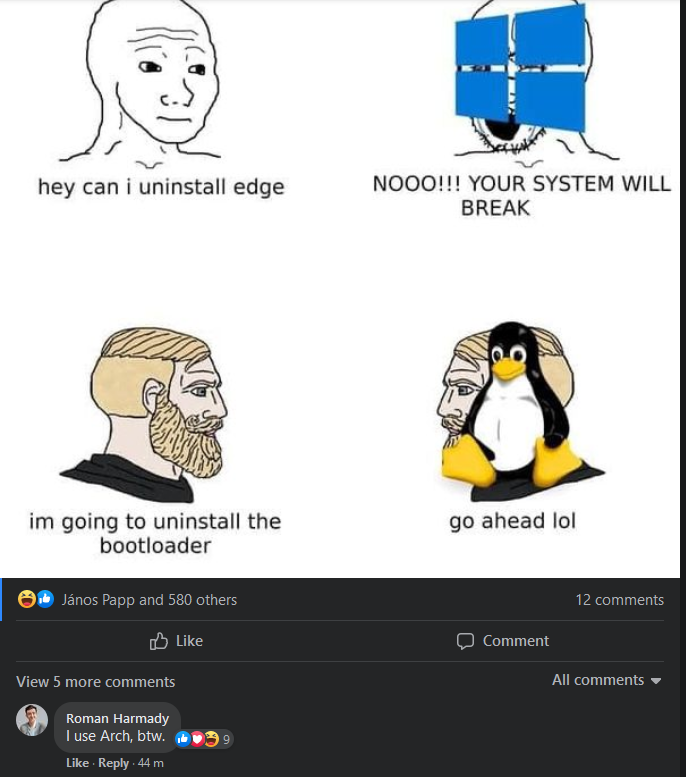
\includegraphics[width=0.9\textwidth]{images/archbtw.png}
	\end{figure}
\end{columns}
\end{frame}